\hsection{Metaheuristics: Why do we need them?}%
%
The main topic of this book will be metaheuristic optimization (although I will eventually also discuss some other methods (remember: work in progress).
So why do we need metaheuristic\indexi{metaheuristics} algorithms?
Why should you read this book?%
%
\hsection{Good Solutions within Acceptable Runtime}%
\label{sec:approximationOfTheOptimum}%
%
The first and foremost reason is that they can provide us good solutions within reasonable time.
It is easy to understand that there are some problems which are harder to solve than others.
Every one of us already knows this from the mathematics classes in school.
Of course, the example problems discussed before cannot be attacked as easily as solving a single linear equation.
They require algorithms, they require computer science.

Ever since primary school, we have learned many problems and types of equations that we can solve.
Unfortunately, theoretical computer science shows that for many problems, the time we need to find the best-possible solution can grow \emph{exponentially}\index{exponential growth} with the number of involved variables in the worst case.
The number of involved variables here could be the number of cities in a \indexi{TSP}, the number of jobs or machines in a \indexi{JSSP}, or the number of objects to pack in a, well, packing problem.
A big group of such complicated problems are called \NPhard~\cite{LLRKS1993SASAAC,CPW1998AROMSCAAA}.
Unless some unlikely breakthrough happens in terms of which problems can be solved efficiently and which not~\cite{C1971TCOTPP,K1972RACP}, there will be many problems that we cannot always solve exactly within reasonable time.
Each and every one of the example problems discussed belongs to this type!

\begin{figure}%
\centering%
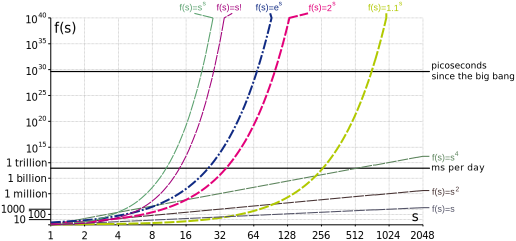
\includegraphics[width=0.99\linewidth]{\currentDir/function_growth}%
\caption{The growth of different functions in a log-log scaled plot. Exponential functions grow very fast. This means that an algorithm which needs~$\sim 2^s$ steps to solve an optimization problem of size~$s$ quickly becomes infeasible if~$s$ grows.}%
\label{fig:function_growth}%
\end{figure}

As sketched in \autoref{fig:function_growth}, the exponential function\index{exponential growth} rises very quickly.
One idea would be to buy more computers for bigger problems and to simply parallelize the computation.
Well, parallelization can provide a linear speed-up at best.
If we have two CPU cores, we can solve the problem in half of the time and if we have three CPU cores, we can do it in one third of the time, and so on {\dots} if the problem lends itself to parallelization (and not all of them do).
Either way, we are dealing with problems where the runtime requirements may double every time we add a single new decision variable.
And no: Quantum computers are not the answer.
Most likely, they cannot even solve these problems qualitatively faster either~\cite{A2008TLOQC}.

So what can we do to solve such problems?
The exponential time requirement occurs if we make \emph{guarantees} about the solution quality, especially about its optimality, over all possible scenarios.
What we can do, therefore, is that we can trade-in the \emph{guarantee} of finding the best possible solution for lower runtime requirements.
We can use algorithms from which we \emph{hope} that they find a good \emph{approximation} of the optimum, i.e., a solution which is very good with respect to the objective function, but which do not \emph{guarantee} that this result will be the best possible solution.
We may sometimes be lucky and even find the optimum, while in other cases, we may get a solution which is close enough.
And we will get this within acceptable time limits.

\begin{figure}%
\centering%
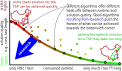
\includegraphics[width=0.9\linewidth]{\currentDir/runtime_quality_tradeoff}%
\caption{The trade-off between solution quality and runtime.}%
\label{fig:runtime_quality_tradeoff}%
\end{figure}

In \autoref{fig:runtime_quality_tradeoff} we illustrate this idea on the example of the \indexi{Traveling Salesperson Problem}\index{TSP}~\cite{ABCC2006TTSPACS,LLRKS1985TTSPAGTOCO,GP2002TTSPAIV} briefly mentioned in \autoref{sec:intro:logistics}.
The goal of solving the TSP is to find the shortest round trip tour through $n$~cities.
The TSP is \NPhard~\cite{GJ1979CAIAGTTTONC,GP2002TTSPAIV}. 
Today, it is possible to solve many large instances of this problem to optimality by using sophisticated \emph{exact} algorithms~\cite{CEG2007CWDPIFTSPT,C2021WT}.
Yet, finding the \emph{shortest possible tour} for a particular TSP might still take many years if you are unlucky.
Finding just \emph{one tour} is, however, very very easy:
I can write down the cities in any particular order.
Of course, I can visit the cities in an arbitrary order.
That is an entirely valid solution, and I can obtain it basically in 0~time.
This \inQuotes{tour} would probably be very bad, very long, and generally not a good idea.

In the real world, we need something in between.
We need a solution which is as good as possible as fast as possible.
Heuristic and metaheuristic algorithms offer different trade-offs of solution quality and runtime.
Different from exact algorithms, they do not guarantee to find the optimal solution and often make no guarantee about the solution quality at all.
Still, they often allow us to get very good solutions for computationally hard problems in short time.
They may often still discover them (just not always, not guaranteed).%
\endhsection%
%
\hsection{Good Solutions within Acceptable Development Time}%
%
Saying that we need a good algorithm to solve a given problem is very easy.
Developing a good algorithm to solve a given problem is not, as any graduate student in the field can probably confirm.
Before, I stated that great exact algorithms for the \indexi{TSP} exist~\cite{CEG2007CWDPIFTSPT,C2021WT}, that can solve many TSPs quickly (although not all).
There are years and years of research in these algorithms.
Even the top heuristic and metaheuristic algorithm for the TSP today result from many years of targeted research~\cite{H2009GKOSFTLKTH,NK2013APGAUEACFTTSP,W2016BNMDPCADIM} and their implementation from the algorithm specification alone can take months~\cite{WWLC2019IIIOADTM}.
Unfortunately, if you do not have plain TSP, but one with some additional constraints --- say, time windows to visit certain cities --- the optimized, state-of-the-art TSP solvers are no longer applicable.
And in a real-world application scenario, you do not have years to develop an algorithm.
What you need are simple, versatile, general algorithm concepts that you can easily adapt to your problem at hand.
Something that can be turned into a working prototype within a few weeks.

Metaheuristics\index{metaheuristics} are the answer~\cite{W2009GOATAA,MF2004HTSIMH}.
They are general algorithm concepts into which we can plug problem-specific modules.
General metaheuristics are usually fairly easy to implement and deliver acceptable results.
Once a sufficiently well-performing prototype has been obtained, we could go and integrate it into the software ecosystem of the customer.
We also can try to improve its performance using different ideas {\dots} and years and years of blissful research, if we are lucky enough to find someone paying for it.%
\endhsection%
\endhsection%
%

